\documentclass{standalone}

\usepackage{tikz}
\usetikzlibrary{er,chains}

\begin{document}
  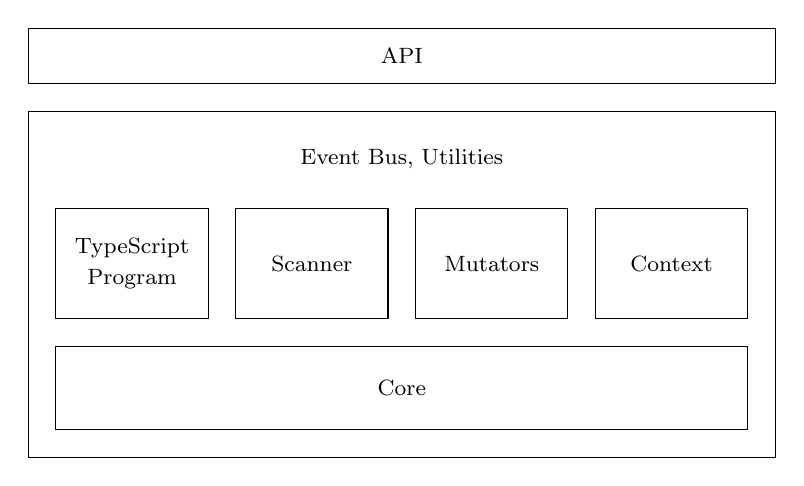
\begin{tikzpicture}[
    auto,
    node distance=1em and 1em,
    font=\footnotesize,
    text centered,
    every entity/.style={
      minimum width=5.5em,
  	  minimum height=4em,
      outer sep=0,
      inner ysep=.5em
    }
  ]
  
  \node [entity] (X) [minimum width=27em, minimum height=12.5em] {};
  
  \node [entity] (Y) [above=of X, minimum width=27em, minimum height=2em] {API};
  
  \node [entity] (A) [above=of X.south, minimum width=25em,minimum height=3em] {Core};
	
  \node [entity] (B) [above=of A.north west,anchor=south west,inner xsep=0] {\begin{tabular}{c}TypeScript\\[.2em]\centering{Program}\end{tabular}};
  \node [entity] (C) [right=of B] {Scanner};
  \node [entity] (D) [right=of C] {Mutators};
  \node [entity] (E) [right=of D] {Context};
  
  \node at (X.north) [rectangle] (t1) [anchor=north,yshift=-1em] {Event Bus, Utilities};
  
  \end{tikzpicture}
\end{document}